\documentclass[border=0.9cm]{standalone}

\usepackage{tikz}
\usetikzlibrary{automata, arrows.meta, positioning}

\begin{document}

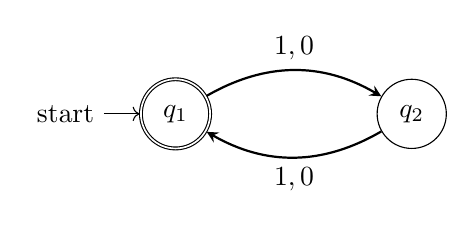
\begin{tikzpicture} [node distance = 3cm, on grid, auto]

\node (q1) [state, accepting, initial] {$q_1$};
\node (q2) [state, right = of q1] {$q_2$};

\path [-stealth, thick]
    (q1) edge[bend left] node {$1,0$} (q2)
    (q2) edge[bend left] node {$1,0$} (q1);
\end{tikzpicture}

\end{document}
